\documentclass[main.tex]{subfiles}


\begin{document}


\section{Results}
\label{results}


\subsection{Strategy of SEARCH-MaP and SEISMIC-RNA}

% In Figure 1, the RNA sequence is CAAUGUGCCAAAGGUCAU (18 nt).
% This sequence could fold into the structures
% ..(((..((...)).))) [P--R interaction formed] and
% ((...))((...)).... [P--R interaction unformed].
% Since its purpose is only to illustrate a toy example, this sequence is never specified in the paper.

\begin{figure}[H]
	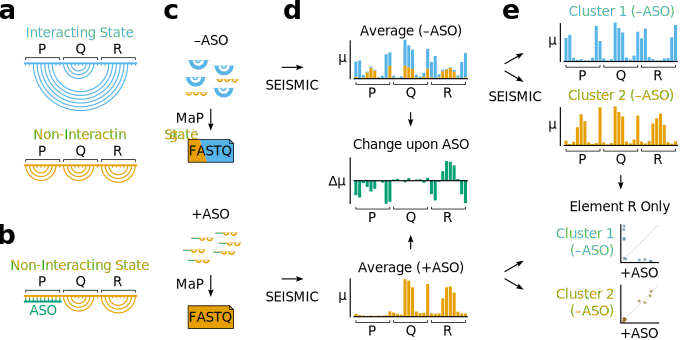
\includegraphics[width=\textwidth]{../MainFigures/strat.pdf}
	\caption{\textbf{The strategy of SEARCH-MaP and SEISMIC-RNA.} \textbf{(a)}~This toy RNA is partitioned into three sections (P, Q, and R) whose molecules exist in two structural states: one in which an interaction between P and R forms (blue) and one in which it does not (purple). \textbf{(b)}~Hybridizing an ASO (red) to P blocks it from interacting with R and forces all RNA molecules into the state where the P--R interaction is unformed. \textbf{(c)} A SEARCH-MaP experiment entails separate chemical probing and mutational profiling (MaP) with (+ASO) and without (--ASO) the ASO, followed by sequencing to generate FASTQ files. The RNA molecules and FASTQ files use the same color scheme as in (a) and are illustrated/colored in proportion to their abundances in the ensemble. \textbf{(d)} Ensemble average mutational profiles with (+ASO) and without (--ASO) the ASO, computed with SEISMIC-RNA. The \textit{x}-axis is the position in the RNA sequence; the \textit{y}-axis is the fraction of mutations ($\mu$) at the position. Each bar in the --ASO profile is drawn in two colors merely to illustrate how much each structural state contributes to each position; in a real experiment, states cannot be distinguished before clustering. The change upon ASO binding (green) indicates the difference in the fraction of mutations ($\Delta \mu$) between the +ASO and --ASO conditions. \textbf{(e)} Mutational profiles of two clusters (top) obtained by clustering the --ASO ensemble in (d) using SEISMIC-RNA, and the scatter plot of the mutation rates of bases in R (bottom) between the +ASO ensemble average (\textit{x}-axis) and each cluster (\textit{y}-axis). The expected correlation ($r$) is shown beside each scatter plot.}
	\label{strat}
\end{figure}

We illustrate SEARCH-MaP with an RNA comprising three sections (P, Q, and R) that folds into an ensemble of two structural states: one in which a base-pairing interaction between P and R forms, another in which it does not (Figure~\ref{strat}a).
Searching for sections that interact with P begins with hybridizing an antisense oligonucleotide (ASO) to P, which blocks P from base pairing with any other section, ablating the state in which the P--R interaction forms (Figure~\ref{strat}b).
The RNA is chemically probed separately with (+ASO) and without (--ASO) the ASO, followed by mutational profiling and sequencing, e.g. using DMS-MaPseq~\cite{Zubradt2016} (Figure~\ref{strat}c).

SEISMIC-RNA can detect RNA--RNA interactions by comparing the +ASO and --ASO mutational profiles.
Theoretically, each structural state has its own mutational profile~\cite{Sherpa2015}, but the mutational profile of a single state is not directly observable because all states are physically mixed during the experiment (Figure~\ref{strat}c, top).
Instead, the directly observable mutational profile is the ``ensemble average" -- the average of the states' (unobserved) mutational profiles, weighted by the states' (unobserved) proportions (Figure~\ref{strat}d, top).
Because the structures -- and therefore mutational profiles -- of R differ between the interaction-formed and -unformed states, the ensemble averages of R also differ between the +ASO and --ASO conditions (Figure~\ref{strat}d, middle).
However, this is not the case for element Q, which has the same secondary structure in both states (Figure~\ref{strat}d, middle).
Therefore, one can deduce that P interacts with R -- but not with Q -- because hybridizing an ASO to P alters the mutational profile of R but not of Q.

After identifying RNA--RNA interactions, SEISMIC-RNA can also determine the mutational profiles of the states where the P--R interaction is formed and unformed -- even if their secondary structures are unknown.
Inferring mutational profiles for the interaction-formed and -unformed states requires clustering the --ASO ensemble into two clusters of RNA molecules (Figure~\ref{strat}e, top).
Each cluster has its own mutational profile and corresponds to one structural state, but which cluster corresponds to the interaction-formed (or -unformed) state is not yet known.
The interaction-unformed state has a mutational profile similar to that of the +ASO ensemble average, since the ASO blocks the interaction and forces the RNA into the interaction-unformed state.
Therefore, a cluster that correlates well ($r \approx 1$) with the +ASO ensemble average (here, Cluster 2) corresponds to the interaction-unformed state; while a cluster that correlates weakly ($r \ll 1$) corresponds to the interaction-formed state (Figure~\ref{strat}e, bottom).


\subsection{(I hope) SEARCH-MaP detects long-range base-pairing in ribosomal RNA}


\subsection{}

Long-range RNA--RNA interactions in many species of virus regulate core processes such as viral protein synthesis~\cite{Nicholson2014}.

In SARS coronavirus 2 (SARS-CoV-2), the frameshift stimulating element (FSE) was shown to base pair with another genomic element over 1,000 nt downstream, a structure the authors named the "FSE-arch"~\cite{Ziv2020}.
We had found that about 45\% of the genomic RNA molecules within infected cells have DMS mutational profiles consistent with the FSE-arch~\cite{Lan2022}, which had surprised us given the length of this RNA--RNA interaction.
Therefore, we sought to investigate and potentially improve the model of the FSE-arch using SEARCH-MaP.

We \textit{in vitro} transcribed a 2,924 nt RNA segment of the SARS-CoV-2 genome centered on the long-range interaction (Figure \ref{tiles}a).
We added groups of DNA ASOs; each group targeted a different section of the RNA (Figure \ref{tiles}a).
Groups 9 and 10 targeted the 3' side of the FSE-arch; we expected that if this structure exists, then adding either group should block part of the FSE-arch and change the structure near the FSE.
We confirmed the ASOs bound using DMS-MaPseq (SFIG).
We then assessed the structure near the FSE via DMS-MaPseq with RT-PCR primers flanking the FSE, including the entire 5' side of the FSE-arch.

The mutational profiles of the FSE region with no ASOs were highly reproducible: the Pearson correlation coefficient (PCC) between two replicates was 0.98 (Figure \ref{tiles}b, light gray).
Binding ASO group F (targeting the FSE itself) plunged the correlation with the no-ASO control to 0.55 (Figure \ref{tiles}b, dark gray), confirming that we could detect ASO-induced structural changes around the FSE.
Of the other ASO groups, only the addition of group 9 dropped the correlation with the no-ASO control below 0.90 (Figure \ref{tiles}b).
This drop in correlation localized to the stems predicted to be part of the FSE-arch (SFIG, on rolling correlation).
This result supports the inner two stems of the FSE-arch.
That adding ASO group 10 had no effect on the FSE (PCC = 0.97) suggests that the outer stem either does not exist or forms less often or under more specific conditions than do the inner two stems.

We next sought to determine in what fraction of molecules the inner two stems of the FSE-arch fold.
We clustered the reads for the no-ASO control using SEISMIC-RNA and found that they form at least two distinct clusters.
These clusters were consistent with our previous data in Vero and Huh-7 cells~\cite{Lan2022} (SFIG), showing that this RNA segment adequately models of the RNA structure in the full-length virus.
We compared the mutational profile of each cluster to that of the ensemble average after adding ASO group 9 (Figure \ref{tiles}c, top).
Cluster 2 (57\% of the ensemble) was very similar (PCC = 0.95), suggesting that this cluster corresponds to the FSE-arch unformed.
Cluster 1 (43\% of the ensemble) was distinct (PCC = 0.64), suggesting that it corresponds to the the FSE-arch formed.

To gain further support for these assignments, we took advantage of having a preexisting model of the FSE-arch~\cite{Ziv2020}.
If these assignments were true, then the mutational profile of Cluster 1 should agree well with the structure of the FSE-arch (i.e. paired and unpaired bases should have low and high mutation rates, respectively); and Cluster 2 should agree less.
We assessed the agreement by constructing a receiver operating characteristic (ROC) curve with respect to the inner two stems of the preexisting model (Figure \ref{tiles}c, bottom).
The area under the curve (AUC) for Cluster 1 was 1.0, indicating perfect agreement with the inner two stems of the FSE-arch, while that of Cluster 2 (AUC = 0.57) was only marginally better than the null expectation of 0.50.
This result supports that Cluster 1 is the mutational profile when the inner two stems of the FSE-arch form, and Cluster 2 when they do not.

If the FSE-arch exists, then blocking the 5' side of the FSE-arch should also alter the structure of the 3' side.
We investigated by RT-PCRing the region surrounding the inner two stems of the FSE-arch on the 3' side with and without adding ASO group F, which targets the FSE.
Similar to the previous result, we found that the 3' side of the FSE-arch also forms two clusters of roughly even proportions (Figure \ref{tiles}d).
The mutational profile (ignoring one outlier) of Cluster 2 resembled blocking the FSE-arch (PCC = 0.95), while Cluster 1 did not (PCC = 0.80); and Cluster 1 agreed with the FSE-arch model (AUC = 1.0), while Cluster 2 did not (AUC = 0.57).
Thus, the 3' side of the FSE-arch also appears to form two structural states, one of which corresponds to the long-range interaction forming.

We conclude that this 2,924 nt segment mimics the FSE-arch in cells and exists as a structure ensemble in which the inner two stems of the FSE-arch fold in 47\% ± 4\% of the molecules (Figure \ref{tiles}e).
As this structure folds \textit{in vitro}, it depends on the RNA sequence itself, not on proteins or other cellular/viral factors.
Moreover, we generated a mutational profile of the formed and the unformed states on both sides of the FSE-arch, which could assist with structure modeling.

\begin{figure}[ht]
	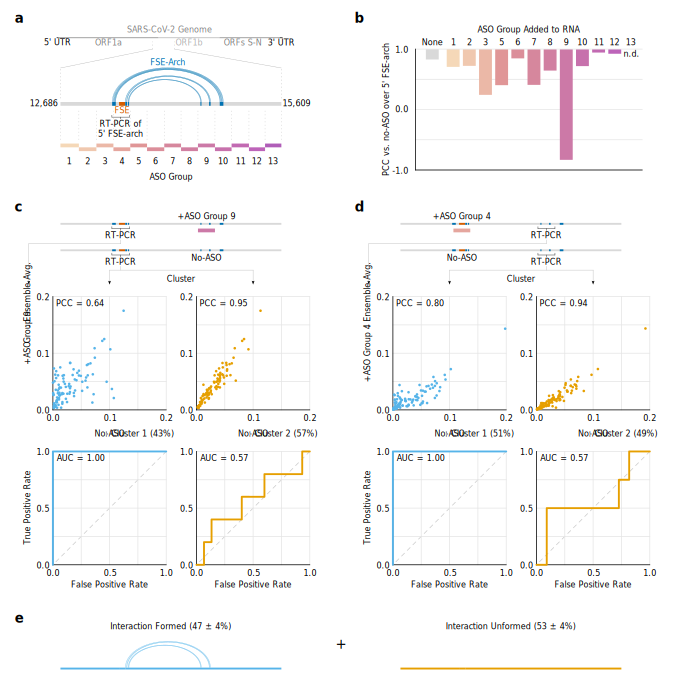
\includegraphics[width=\textwidth]{../MainFigures/sars2-tile/sars2-tile.pdf}
	\caption{}
	\label{tiles}
\end{figure}



\subfile{covs}
\subfile{tgev}


\end{document}
